\documentclass{article}
\usepackage{graphicx}
\usepackage{amsmath}
\usepackage{listings}
\usepackage{geometry}
\usepackage{physics}
\usepackage[utf8]{inputenc}

\geometry{
 a4paper,
 total={170mm,257mm},
 left=20mm,
 top=20mm,
 }

\title{Assignment7}
\author{Jineeth N [EE20B051]}
\date{April 8,2022}

\begin{document}

\maketitle

\section{Introduction}
This assignemnt involves the analysis of filters using Laplace Transforms. Python's symbolic solving library, Sympy is used to solve Modified Nodal Analysis equations. Scipy library is used to calculate output responses of the systems

\section*{Low Pass Filter}
The low pass filter that we use gives the following matrix equation after simplification of the modified nodal equations.
\[\begin{pmatrix} 0 & 0 & 1 & -\frac{1}{G} \\ -\frac{1}{1+sR_2C_2} & 1 & 0 & 0 \\ 0 & -G & G & 1 \\ -\frac{1}{R_1}-\frac{1}{R_2}-sC_1 & \frac{1}{R_2} & 0 & sC_1 \end{pmatrix}\begin{pmatrix} V_1 \\ V_p \\ V_m \\ V_o \end{pmatrix} = \begin{pmatrix} 0 \\ 0 \\ 0 \\ -V_i(s)/R_1 \end{pmatrix}\]
Below is the code for Low Pass Filter
\begin{verbatim}

    def lowpass(R1, R2, C1, C2, G, Vi):
    s = symbols("s")
    # Creating the matrices and solving them to get the output voltage.
    A = Matrix(
        [
            [0, 0, 1, -1 / G],
            [-1 / (1 + s * R2 * C2), 1, 0, 0],
            [0, -G, G, 1],
            [-1 / R1 - 1 / R2 - s * C1, 1 / R2, 0, s * C1],
        ]
    )
    b = Matrix([0, 0, 0, -Vi / R1])
    V = A.inv() * b
    return A, b, V

        
\end{verbatim}

\begin{figure}[!ht]
  \centering
  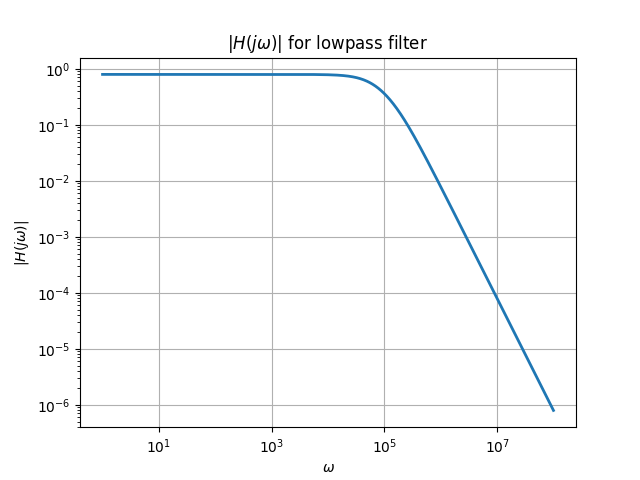
\includegraphics[scale=0.5]{Figure_0.png}
  \caption{Magnitude response of Low Pass filter}
  \label{fig:sample}
  \end{figure}

\newpage
\section*{High Pass Filter}
The high pass filter we use gives the following matrix equations after simplification of the modified nodal equations
\[\begin{pmatrix} 0 & 0 & 1 & -\frac{1}{G} \\ -\frac{-sR_3C_2}{1+sR_3C_2} & 1 & 0 & 0 \\ 0 & -G & G & 1 \\ -1-(sR_1C_1)-(sR_3C_2)) & sC_2R_1 & 0 & 1 \end{pmatrix}\begin{pmatrix} V_1 \\ V_p \\ V_m \\ V_o \end{pmatrix} = \begin{pmatrix} 0 \\ 0 \\ 0 \\ -V_i(s)sR_1C_1 \end{pmatrix}\]
Below is the code for High Pass Filter
\begin{verbatim}
    def highpass(R1, R3, C1, C2, G, Vi):
    s = symbols("s")
    # Creating the matrices and solving them to get the output voltage.
    A = Matrix(
        [
            [0, -1, 0, 1 / G],
            [s * C2 * R3 / (s * C2 * R3 + 1), 0, -1, 0],
            [0, G, -G, 1],
            [-s * C2 - 1 / R1 - s * C1, 0, s * C2, 1 / R1],
        ]
    )
    b = Matrix([0, 0, 0, -Vi * s * C1])
    V = A.inv() * b
    return A, b, V
\end{verbatim}

\begin{figure}[!ht]
  \centering
  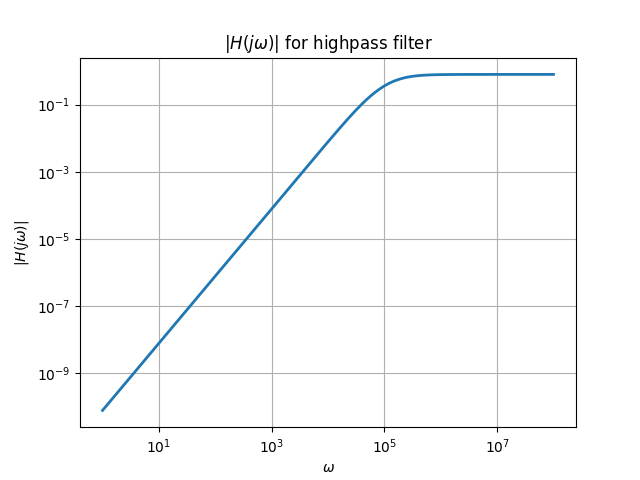
\includegraphics[scale=0.5]{Figure_3.png}
  \caption{Magnitude response of High Pass filter}
  \label{fig:sample}
  \end{figure}

\newpage
\section{Tasks}
\subsection{Step response Low Pass Filter}
    Output Voltage for unit step function as an input

\begin{verbatim}
   # These lines of code will calculate the step response for the lowpass filter.
A1, b1, V1 = lowpass(10000, 10000, 1e-9, 1e-9, 1.586, 1 / s)
Vo1 = V1[3]
H1 = sympyToCoeff(Vo1)
t, y1 = sp.impulse(H1, None, p.linspace(0, 5e-3, 10000))

# The plot for step response of a lowpass filter.
plt.figure(1)
plt.plot(t, y1)
plt.title(r"Step Response for low pass filter", fontsize=12)
plt.xlabel(r"$t$", fontsize=10)
plt.ylabel(r"$V_o(t)$", fontsize=10)
plt.grid(True)
\end{verbatim}

\begin{figure}[!ht]
  \centering
  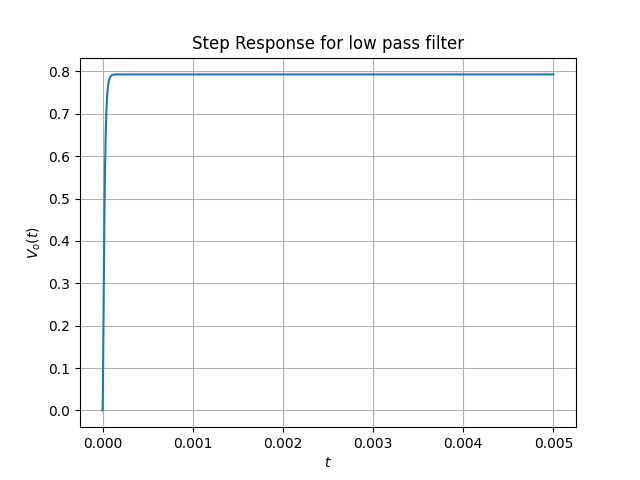
\includegraphics[scale=0.7]{Figure_1.png}
  \caption{Step response of Low Pass filter}
  \label{fig:sample}
  \end{figure}
  
\subsection{Response to sum of sinusoids}
 Input function is,
\begin{equation*}
  V_{i}(t) = ( \ \sin(2000\pi t) + \cos(2*10^{6}\pi t) \ )u_{o}(t) \ Volts
  \end{equation*}
Output response for the Low Pass filter can be found as shown in the code snippet.
\begin{verbatim}
        # The response is also calculated for sum of sinusoids.
    a = 2e3
    b = 2e6
    vi = p.sin(a * PI * t) + p.cos(b * PI * t)
    t, y2, svec = sp.lsim(H, vi, t)
    
    # The plot for output response for sum of sinusoids of a lowpass filter.
    plt.figure(2)
    plt.plot(t, y2)
    plt.title(r"Output voltage for sum of sinusoids", fontsize=12)
    plt.xlabel(r"$t$", fontsize=10)
    plt.ylabel(r"$V_o(t)$", fontsize=10)
    plt.grid(True)
\end{verbatim}

\begin{figure}[!ht]
  \centering
  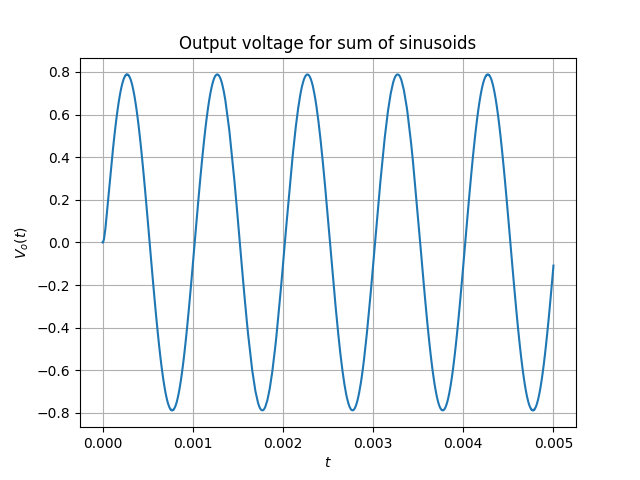
\includegraphics[scale=0.7]{Figure_2.png}
  \caption{Output Voltage for sum of sinusoids}
  \label{fig:sample}
  \end{figure}
  
\subsection{Response to damped sinusoid}
In this case we assign the input voltage as a damped sinusoid like,\\
Low frequency,
\begin{equation*}
    V_{i}(t) = e^{-500t}( \ \cos(2000\pi t) \ )u_{o}(t) \ V
\end{equation*}
High frequency,
\begin{equation*}
    V_{i}(t) = e^{-500t}( \ \cos(2*10^{6}\pi t) \ )u_{o}(t) \ V
\end{equation*}

\subsubsection{High Pass filter response}
Below is the code for calculating output of High Pass filter for damped sin functions
\begin{verbatim}
    # The below piece of code will calculate the transfer function for the highpass filter.
A3, b3, V3 = highpass(10000, 10000, 1e-9, 1e-9, 1.586, 1)
Vo3 = V3[3]
H3 = sympyToCoeff(Vo3)
hf3 = lambdify(s, Vo3, "numpy")
v3 = hf3(ss)

\end{verbatim}

\newpage
Output for Low and High frequency inputs

\begin{figure}[!ht]
  \centering
  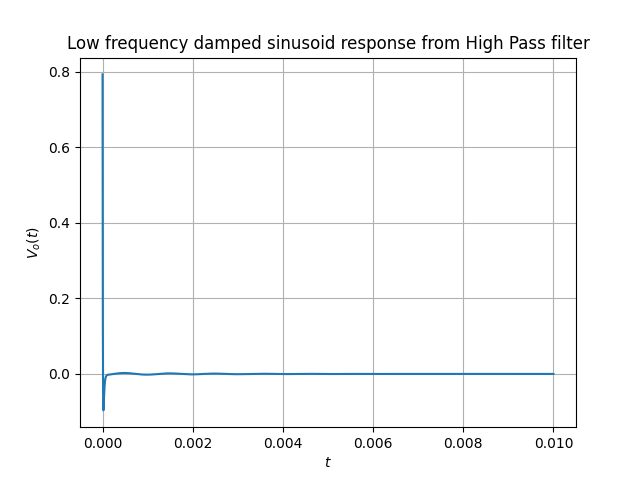
\includegraphics[scale=0.7]{Figure_7.png}
  \caption{Output for Low frequency sinusoid}
  \label{fig:sample}
  \end{figure}
  
\begin{figure}[!ht]
  \centering
  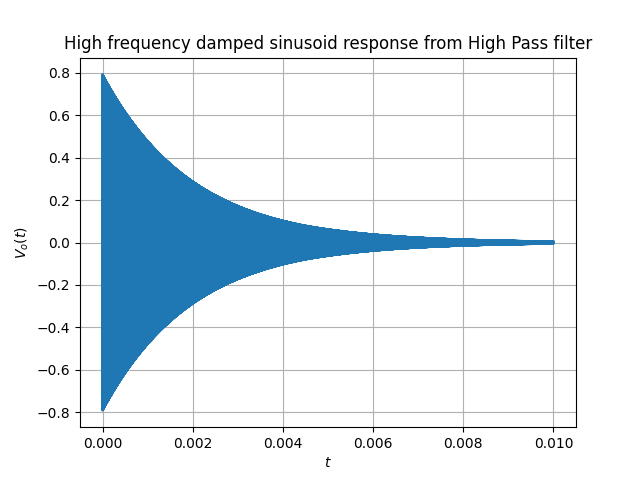
\includegraphics[scale=0.7]{Figure_6.png}
  \caption{Output for High frequency sinusoid}
  \label{fig:sample}
  \end{figure}
  
  
\subsubsection{Low Pass filter response}
Below is the code for calculating output of Low Pass filter for damped sin functions

\begin{verbatim}
    A4, b4, V4 = lowpass(10000, 10000, 1e-9, 1e-9, 1.586, 1)
Vo4 = V4[3]
H4 = sympyToCoeff(Vo4)
hf3 = lambdify(s, Vo4, "numpy")
v3 = hf3(ss)

\end{verbatim}

\begin{figure}[!ht]
  \centering
  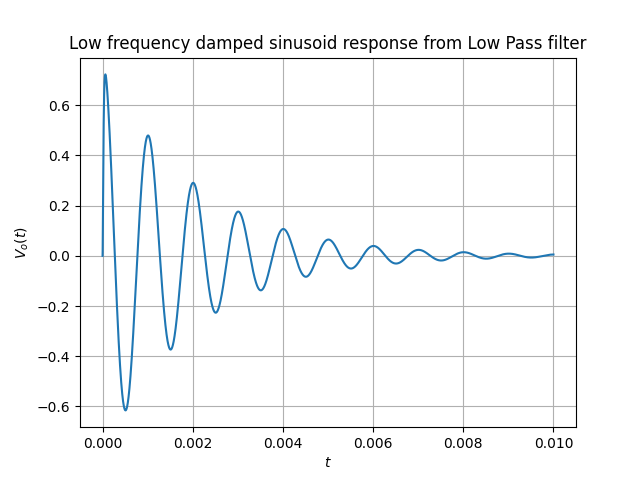
\includegraphics[scale=0.7]{Figure_10.png}
  \caption{Output for Low frequency sinusoid}
  \label{fig:sample}
  \end{figure}
  
\begin{figure}[!ht]
  \centering
  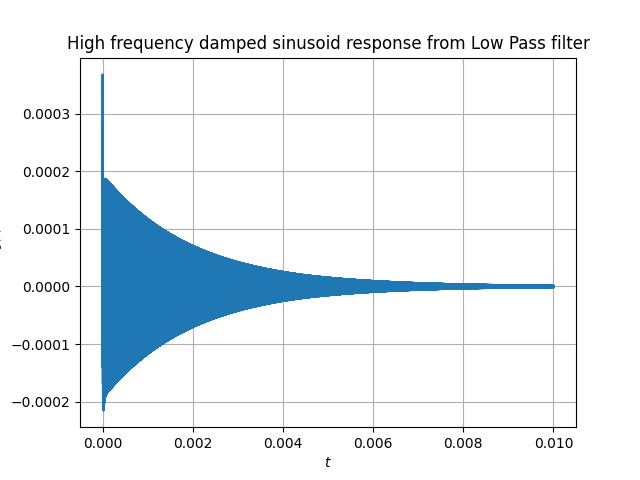
\includegraphics[scale=0.7]{Figure_9.png}
  \caption{Output for High frequency sinusoid}
  \label{fig:sample}
  \end{figure}

\newpage
\subsection{Step Response of High Pass filter}
Step response can be calculated by substituting, $ Vi(s) = 1/s $.

\begin{verbatim}
    A5, b5, V5 = highpass(10000, 10000, 1e-9, 1e-9, 1.586, 1 / s)
Vo5 = V5[3]
H5 = sympyToCoeff(Vo5)
t, y5 = sp.impulse(H5, None, p.linspace(0, 5e-3, 10000))
\end{verbatim}

\begin{figure}[!ht]
  \centering
  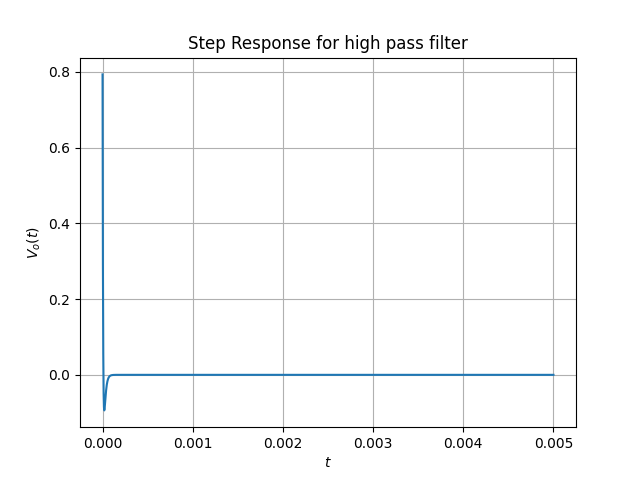
\includegraphics[scale=0.7]{Figure_11.png}
  \caption{Output for High frequency sinusoid}
  \label{fig:sample}
  \end{figure}

\newpage
\section{Conclusion}

 The sympy module has allowed us to analyse circuits by analytically solving their node equations. And we used signal toolbox in python to find the time domain responses of the frequency responses
\end{document}
